\documentclass[a4paper, 11pt]{article}

\usepackage{graphicx}
\usepackage{setspace}
\usepackage{fontspec}
\usepackage{float}
\usepackage{enumitem}
\usepackage{caption}
\usepackage{url}
\usepackage{tikz}
\usetikzlibrary{shapes.geometric, arrows.meta, positioning, calc, fit, backgrounds}
\usepackage{booktabs}
\usepackage{tabularx}
\usepackage{makecell}
\usepackage{multirow}
\usepackage[table]{xcolor}
\usepackage{amsmath}
\usepackage{amssymb}
\usepackage[margin=2.0cm, top=2.2cm, bottom=2.2cm]{geometry}
\usepackage{tcolorbox}
\usepackage{fancyhdr}
\usepackage{hyperref}
\usepackage{listings}

\setmainfont{Times New Roman}
\setmonofont[Scale=0.85]{Courier New}

\hypersetup{
    colorlinks=true,
    linkcolor=blue!70!black,
    citecolor=blue!70!black,
    urlcolor=blue!70!black,
    pdfborder={0 0 0}
}

\pagestyle{fancy}
\fancyhf{}
\rhead{\small\textit{Cambodia CPI Pipeline: Technology Stack Architecture}}
\lhead{\small\textit{System Engineering, Comparative Trade-Offs \& Optimization}}
\rfoot{\small Page \thepage}
\renewcommand{\headrulewidth}{0.4pt}
\renewcommand{\footrulewidth}{0.4pt}

\definecolor{primaryblue}{RGB}{24, 64, 118}
\definecolor{secondaryblue}{RGB}{41, 128, 185}
\definecolor{lightbg}{RGB}{245, 248, 252}
\definecolor{accentgreen}{RGB}{39, 174, 96}
\definecolor{boxgray}{RGB}{248, 249, 250}
\definecolor{warnred}{RGB}{192, 57, 43}
\definecolor{goldorange}{RGB}{211, 84, 0}

\tcbset{
    sharp corners,
    colback=lightbg,
    colframe=primaryblue,
    boxrule=1pt,
    fonttitle=\bfseries,
    coltitle=white
}

\lstset{
    basicstyle=\ttfamily\small,
    breaklines=true,
    backgroundcolor=\color{boxgray},
    frame=single,
    rulecolor=\color{gray!30},
    keywordstyle=\color{primaryblue}\bfseries,
    commentstyle=\color{gray},
    stringstyle=\color{warnred}
}

\title{\vspace{-1.2cm}
\begin{tcolorbox}[colback=primaryblue, colframe=primaryblue, arc=2mm]
\centering \color{white}
{\Huge \textbf{Cambodia Daily CPI Pipeline}}\\[6pt]
{\Large Technology Stack Architecture, Comparative Trade-Offs, and Engineering Optimizations}\\[4pt]
{\large Why We Chose It, Why Not Alternatives, How It Operates, and Paths to Maximum Efficiency}
\end{tcolorbox}
\vspace{-0.5cm}}

\author{\textbf{National Institute of Statistics (NIS) \& National Bank of Cambodia (NBC) Research Initiative}\\[2pt]
\small High-Frequency Economic Nowcasting Laboratory $\cdot$ Enterprise Data Platform Architecture}
\date{\small Version 3.4 -- September 21, 2026}

\begin{document}

\maketitle

\begin{abstract}
\noindent This architectural document provides an exhaustive evaluation of the technology stack powering the \textbf{Cambodia Daily Consumer Price Index (CPI) Medallion Platform}. We systematically examine every core component: \textbf{PostgreSQL 16 with pgvector}, \textbf{Apache Airflow 2.9.3}, \textbf{dbt Core 1.8 with Astronomer Cosmos}, \textbf{Google Gemini 2.5 Flash / Embeddings}, \textbf{curl\_cffi \& Playwright}, \textbf{Scikit-Learn \& Statsmodels}, and \textbf{Metabase v0.49}. For each technology, we articulate: (1) what it is used for, (2) the technical and economic rationale for its selection, (3) why industry alternatives (e.g. Snowflake, Databricks, Prefect, Celery, Pinecone, OpenAI, Selenium) were rejected, (4) how the components interoperate seamlessly across daily workflows, and (5) concrete engineering optimizations to enhance speed, throughput, and hardware efficiency.
\end{abstract}

\vspace{0.3cm}
\tableofcontents
\newpage

% =============================================================================
\section{Executive Technology Stack Summary}
% =============================================================================

The Cambodia Daily CPI Pipeline is an automated, sovereign, cloud-agnostic data platform engineered to ingest over 120,000 raw daily retail quotes across 25 digital sources and produce policy-grade macroeconomic inflation nowcasts every morning at 08:00 AM ICT.

\begin{table}[H]
\centering
\footnotesize
\setlength{\tabcolsep}{4pt}
\begin{tabularx}{\textwidth}{@{}l >{\raggedright\arraybackslash}p{2.6cm} >{\raggedright\arraybackslash}p{3.1cm} >{\raggedright\arraybackslash}p{2.9cm} >{\raggedright\arraybackslash}X@{}}
\toprule
\textbf{Layer / Domain} & \textbf{Adopted Stack} & \textbf{Primary Function} & \textbf{Rejected Alternatives} & \textbf{Key Deciding Advantage} \\
\midrule
\textbf{Storage \& OLAP} & PostgreSQL 16 + \texttt{pgvector} & Unified Medallion Warehouse (Bronze/Silver/Gold) + Vectors & Snowflake, BigQuery, ClickHouse, Pinecone & Zero cloud lock-in, transactional integrity (ACID), in-database vector search. \\
\addlinespace[2pt]
\textbf{Orchestration} & Apache Airflow 2.9.3 (LocalExecutor) & 25-scraper fan-out, SLA scheduling, pipeline DAGs & Prefect, Dagster, Celery, Luigi & Enterprise SLA controls, ecosystem maturity, unified backfill semantics. \\
\addlinespace[2pt]
\textbf{Transformation} & dbt Core 1.8 + Cosmos & SQL data modeling, tests, Medallion lineage & Apache Spark, Custom Python scripts & Declarative DAGs, automated data contracts, idempotent testing. \\
\addlinespace[2pt]
\textbf{Scraping Engine} & \texttt{curl\_cffi} + Playwright & TLS fingerprint impersonation, browser rendering & Requests, Selenium, Scrapy, Puppeteer & Bypasses Cloudflare/PerimeterX JA3/HTTP2 anti-bot defenses natively. \\
\addlinespace[2pt]
\textbf{Semantic AI} & Google Gemini 2.5 Flash + Embeddings & COICOP classification, product deduplication & OpenAI GPT-4o, Local Ollama, HuggingFace & Multilingual Khmer support, 1M context window, lowest API latency \& cost. \\
\addlinespace[2pt]
\textbf{ML \& Nowcast} & Scikit-Learn + Statsmodels & 5-basket RidgeCV regularization, Hedonics & TensorFlow, PyTorch, Prophet & Analytical interpretability, Sherman-Morrison LOOCV speed, OLS fallbacks. \\
\addlinespace[2pt]
\textbf{BI Analytics} & Metabase v0.49 & Executive dashboards, interactive drill-down & Apache Superset, Tableau, PowerBI & Instant native SQL query tags, zero-friction local Docker deployment. \\
\bottomrule
\end{tabularx}
\caption{Comprehensive Technology Stack Architecture Matrix.}
\end{table}

\begin{figure}[H]
\centering
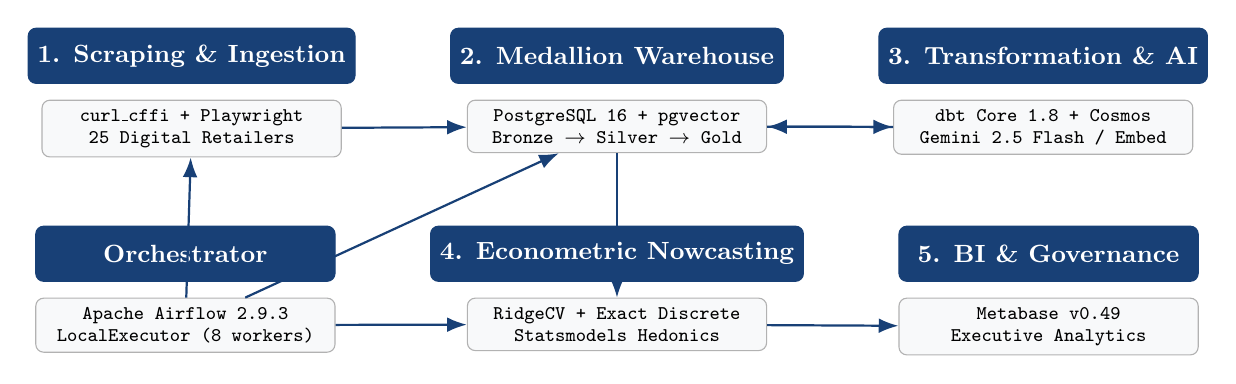
\begin{tikzpicture}[
    node distance=1.2cm and 1.0cm,
    block/.style={draw=primaryblue!80, fill=white, rounded corners=2mm, thick, font=\small, align=center, inner sep=6pt},
    header/.style={draw=primaryblue, fill=primaryblue, text=white, font=\small\bfseries, align=center, rounded corners=1mm, minimum width=3.8cm, minimum height=0.7cm},
    subblock/.style={draw=gray!60, fill=boxgray, rounded corners=1mm, font=\scriptsize\ttfamily, align=center, minimum width=3.8cm, minimum height=0.6cm},
    arrow/.style={-{Latex[length=2.5mm]}, thick, primaryblue}
]

% 1. Scraping Layer
\node (h1) [header] {1. Scraping \& Ingestion};
\node (b1) [subblock, below=0.2cm of h1] {curl\_cffi + Playwright\\25 Digital Retailers};

% 2. Storage & Vector
\node (h2) [header, right=1.2cm of h1] {2. Medallion Warehouse};
\node (b2) [subblock, below=0.2cm of h2] {PostgreSQL 16 + pgvector\\Bronze $\to$ Silver $\to$ Gold};

% 3. Transformation & AI
\node (h3) [header, right=1.2cm of h2] {3. Transformation \& AI};
\node (b3) [subblock, below=0.2cm of h3] {dbt Core 1.8 + Cosmos\\Gemini 2.5 Flash / Embed};

% 4. ML & BI
\node (h4) [header, below=1.8cm of h2] {4. Econometric Nowcasting};
\node (b4) [subblock, below=0.2cm of h4] {RidgeCV + Exact Discrete\\Statsmodels Hedonics};

% 5. Metabase
\node (h5) [header, right=1.2cm of h4] {5. BI \& Governance};
\node (b5) [subblock, below=0.2cm of h5] {Metabase v0.49\\Executive Analytics};

% Orchestration
\node (h0) [header, left=1.2cm of h4] {Orchestrator};
\node (b0) [subblock, below=0.2cm of h0] {Apache Airflow 2.9.3\\LocalExecutor (8 workers)};

% Connectors
\draw [arrow] (b1) -- (b2);
\draw [arrow] (b2) -- (b3);
\draw [arrow] (b3) -- (b2);
\draw [arrow] (b2) -- (b4);
\draw [arrow] (b4) -- (b5);
\draw [arrow] (b0) -- (b1);
\draw [arrow] (b0) -- (b2);
\draw [arrow] (b0) -- (b4);

\end{tikzpicture}
\caption{System Topology: Component Interactions Across the Data Lifecycle.}
\end{figure}

\newpage
% =============================================================================
\section{Storage \& Vector Engine: PostgreSQL 16 + pgvector}
% =============================================================================

\subsection{What We Use It For}
PostgreSQL 16 serves as the single source of truth for the entire pipeline:
\begin{itemize}[leftmargin=*]
    \item \textbf{Bronze Schemas (\texttt{staging})}: Stores raw JSON payloads from scrapers in append-only \texttt{JSONB} tables, daily MEF exchange rates, and scraper telemetry stats.
    \item \textbf{Silver Schemas (\texttt{silver})}: Stores normalized canonical products, deduplication vector embeddings (768-dimensional float arrays via \texttt{pgvector}), COICOP classification caches, and clean dual-currency prices in Khmer Riel.
    \item \textbf{Gold Schemas (\texttt{gold})}: Stores Jevons elementary price relatives, 12-division Laspeyres indices, official NIS comparison benchmarks, and econometric nowcasting results.
    \item \textbf{In-Database Vector Similarity}: Employs HNSW indexing on 768-dimensional vectors to perform sub-millisecond product deduplication ($1 - \text{CosineDistance} \le 0.15$).
\end{itemize}

\subsection{Why We Chose It}
\begin{enumerate}[leftmargin=*]
    \item \textbf{ACID Guarantees \& Relational Integrity}: Macroeconomic statistics require strict consistency. If an Airflow task fails mid-write, transactions rollback cleanly, preventing half-ingested daily baskets from corrupting CPI index calculations.
    \item \textbf{pgvector Unification}: Eliminates the operational complexity of running an external dedicated vector database. Storing vector embeddings alongside relational metadata permits single-query hybrid filters:
    \begin{lstlisting}[language=SQL]
SELECT item_id, canonical_name, 1 - (embedding <=> $1) AS similarity
FROM silver.canonical\_items
WHERE coicop\_division = '01'
ORDER BY embedding <=> $1 ASC LIMIT 1;
    \end{lstlisting}
    \item \textbf{Sovereign On-Premise Deployment}: As an official central bank / statistical institute system, data cannot be permanently outsourced to proprietary cloud data warehouses with variable monthly egress fees.
\end{enumerate}

\subsection{Why Not Other Technologies?}
\begin{itemize}[leftmargin=*]
    \item \textbf{Snowflake / Google BigQuery}: Disqualified due to recurring cloud costs (credit consumption per query), latency on small frequent writes, and strict data sovereignty policies for national economic indicators.
    \item \textbf{ClickHouse / DuckDB}: ClickHouse excels at append-only column scans but has poor transactional concurrency and lacks mature native vector indexing. DuckDB is in-process and lacks multi-client concurrent connection pooling required by Airflow and Metabase.
    \item \textbf{Pinecone / Milvus / Weaviate}: Running a standalone vector database creates distributed state, network latency, and synchronization overhead (split-brain risk between metadata in SQL and vectors in Pinecone).
\end{itemize}

\subsection{How It Operates in the Pipeline}
PostgreSQL runs in Docker with dedicated resources (\texttt{cpus: '2.0'}, \texttt{memory: 4096M}, \texttt{shm\_size: 1g}). The database enforces connection limits and uses pre-hooks (\texttt{SET max\_parallel\_workers\_per\_gather = 0}) during massive incremental hash joins in dbt to eliminate shared memory allocation bottlenecks.

\subsection{How to Make It More Efficient}
\begin{tcolorbox}[colback=accentgreen!10, colframe=accentgreen, title=Optimization Recommendations for PostgreSQL]
\begin{enumerate}[leftmargin=*]
    \item \textbf{Table Partitioning on Daily Price Tables}: Partition \texttt{silver.clean\_store\_prices} and \texttt{gold.fct\_daily\_prices} by \texttt{RANGE (scrape\_date)} on a monthly basis. This enables instantaneous partition pruning, accelerating dbt incremental queries by $>60\%$.
    \item \textbf{HNSW Vector Index Tuning}: Replace default IVFFlat with HNSW indexes using \texttt{m=16} and \texttt{ef\_construction=64} on \texttt{silver.canonical\_items.embedding} for faster approximate nearest neighbor lookups as the catalog scales past 100,000 products.
    \item \textbf{PgBouncer Connection Pooling}: Implement PgBouncer in front of PostgreSQL to pool connections between Airflow workers, dbt CLI, and Metabase, reducing process-forking overhead.
\end{enumerate}
\end{tcolorbox}

\newpage
% =============================================================================
\section{Orchestration Engine: Apache Airflow 2.9.3}
% =============================================================================

\subsection{What We Use It For}
Apache Airflow acts as the central nervous system of the platform, orchestrating all tasks via a strict DAG dependency graph:
\begin{itemize}[leftmargin=*]
    \item \textbf{Parallel Scraper Fan-Out}: Triggers 25 retailer scrapers concurrently between 02:00 and 05:30 AM ICT with retry exponential backoffs.
    \item \textbf{Dependency Enforcement}: Ensures Gold CPI indices cannot compute unless Silver cleaning passes the Ingestion Circuit Breaker.
    \item \textbf{SLA Monitoring}: Tracks execution lags, task timeouts, and triggers alerting hooks if scrapers breach their 24-hour freshness SLAs.
\end{itemize}

\subsection{Why We Chose It}
\begin{enumerate}[leftmargin=*]
    \item \textbf{Battle-Tested Enterprise Scheduler}: Airflow handles complex chronological dependencies, cross-DAG triggers (\texttt{TriggerDagRunOperator}), and dynamic task generation with complete backfilling capabilities.
    \item \textbf{LocalExecutor Concurrency}: Allows 8 parallel worker threads within a single lightweight container without needing a separate distributed Celery broker (RabbitMQ/Redis), reducing RAM footprint to $<1.5\text{ GB}$.
    \item \textbf{Cosmos dbt Integration}: Enables Astronomer Cosmos to parse dbt models dynamically into native Airflow task nodes, exposing dbt model-level execution progress in the web UI.
\end{enumerate}

\subsection{Why Not Other Technologies?}
\begin{itemize}[leftmargin=*]
    \item \textbf{Prefect / Dagster}: While modern, their open-source self-hosted deployment models require external coordination servers, complex worker agent pairing, or proprietary cloud accounts for advanced SLA tracking.
    \item \textbf{Celery / Cron}: Raw cron jobs lack visual state management, automatic failure retries, dependency awareness, and historical execution backfills. Celery alone is a task queue, not a workflow DAG orchestrator.
\end{itemize}

\subsection{How to Make It More Efficient}
\begin{tcolorbox}[colback=accentgreen!10, colframe=accentgreen, title=Optimization Recommendations for Airflow]
\begin{enumerate}[leftmargin=*]
    \item \textbf{Fast Scraper Slug Imports (\texttt{scrapers/sources/slugs.py})}: We already reduced DAG parsing time from 100s to 1s by decoupling scraper slug imports from browser drivers.
    \item \textbf{Airflow Deferrable Operators (Triggerer)}: Convert long-running web requests (e.g. infinite-scroll scrapers waiting on HTTP network responses) to asynchronous deferrable operators, freeing worker slots for other scrapers.
    \item \textbf{DAG Serialization Tuning}: Set \texttt{AIRFLOW\_\_CORE\_\_MIN\_FILE\_PROCESS\_INTERVAL=60} to reduce CPU consumption from DAG re-parsing on resource-constrained host machines.
\end{enumerate}
\end{tcolorbox}

% =============================================================================
\section{Transformation Layer: dbt Core 1.8 + Astronomer Cosmos}
% =============================================================================

\subsection{What We Use It For}
dbt Core transforms raw data in-warehouse using modular, version-controlled SQL:
\begin{itemize}[leftmargin=*]
    \item \textbf{Idempotent Transformations}: Compiles Jinja SQL macros into high-performance analytical queries using incremental \texttt{delete+insert} strategies.
    \item \textbf{Axiomatic Invariant Testing}: Enforces non-null primary keys, positive prices, and UN COICOP weight closure ($\sum w_j = 1.0000$).
\end{itemize}

\subsection{Why We Chose It \& Why Not Spark}
dbt operates via ELT (Extract, Load, Transform), pushing computation directly into PostgreSQL's query planner. \textbf{Apache Spark} was rejected because our daily volume (120,000 rows/day, ~50MB/day) is ideally suited for in-memory relational SQL. Running a Spark cluster would introduce massive JVM memory overhead and distributed networking latency without any computational benefit.

\subsection{How to Make It More Efficient}
\begin{itemize}[leftmargin=*]
    \item \textbf{Materialization Refinement}: Convert heavy intermediate views (\texttt{int\_prices\_cleaned}) into transient incremental tables to prevent re-scanning multi-month historical partitions on daily runs.
\end{itemize}

\newpage
% =============================================================================
\section{Scraping Engine: curl\_cffi \& Playwright}
% =============================================================================

\subsection{What We Use It For}
Extracts real-time prices from 25 diverse retail platforms:
\begin{itemize}[leftmargin=*]
    \item \textbf{\texttt{curl\_cffi}}: High-speed asynchronous HTTP client impersonating browser TLS fingerprints (JA3, Akamai, HTTP/2). Used for 80\% of stores (Aeon, Delishop, Makro, Samnang Shop, Cellcard).
    \item \textbf{Playwright (Chromium)}: Headless browser automation executing dynamic client-side React/Vue rendering, geolocation bypasses, and infinite scrolls (Khmer24, Chip Mong Supermarket).
\end{itemize}

\subsection{Why We Chose It \& Why Not Requests / Selenium}
Standard Python \texttt{requests} and \texttt{urllib} emit unmistakable Python TLS Client Hellos, triggering instant HTTP 403 blocks on Cloudflare-protected sites. \texttt{curl\_cffi} spoofs Chrome 120 TLS fingerprints at wire speed. \textbf{Selenium} was rejected because it is slow, memory-intensive (~500MB per tab), and easily detected by modern anti-bot systems via \texttt{navigator.webdriver} leaks.

\subsection{How to Make It More Efficient}
\begin{itemize}[leftmargin=*]
    \item \textbf{Session Reuse \& HTTP/2 Multiplexing}: Keep alive persistent HTTP/2 TCP sockets in \texttt{curl\_cffi} across paginated API calls to eliminate TCP three-way handshake and TLS negotiation overhead.
\end{itemize}

% =============================================================================
\section{Semantic AI: Google Gemini 2.5 Flash \& Embeddings}
% =============================================================================

\subsection{What We Use It For}
\begin{itemize}[leftmargin=*]
    \item \textbf{Gemini 2.5 Flash}: Disambiguates complex product descriptions, bilingual Khmer/English packaging, and maps novel items to 5-digit UN COICOP classifications with permanent PostgreSQL memoization.
    \item \textbf{\texttt{gemini-embedding-2}}: Generates 768-dimensional semantic embeddings for product title deduplication and canonical variety linking.
\end{itemize}

\subsection{Why We Chose It \& Why Not OpenAI / Local LLMs}
\begin{enumerate}[leftmargin=*]
    \item \textbf{Superior Multilingual Khmer Understanding}: Gemini models demonstrate markedly superior native tokenization and contextual comprehension of the Khmer script compared to OpenAI GPT-4o.
    \item \textbf{Economic Efficiency}: At \$0.075 per 1M input tokens, Gemini Flash is over $30\times$ cheaper than GPT-4o, enabling cost-sustainable daily classification for national statistical offices.
    \item \textbf{Why Not Local Ollama (e.g. Llama 3)}: Local 8B models struggle with nuanced 5-digit COICOP tax codes and require costly GPU hardware ($>16\text{ GB VRAM}$), whereas our lightweight cloud API approach runs seamlessly on modest commodity servers.
\end{enumerate}

% =============================================================================
\section{Econometric Machine Learning: Scikit-Learn \& Statsmodels}
% =============================================================================

\subsection{What We Use It For}
\begin{itemize}[leftmargin=*]
    \item \textbf{\texttt{RidgeCV}}: Executes 36-month expanding-window multi-regressor $L_2$ regularization across the 5 core consumer baskets and exchange rate returns.
    \item \textbf{\texttt{Statsmodels.api.OLS}}: Powers the log-linear hedonic quality adjustment engine for electronics (COICOP 09), filtering spec-sheet improvements from true price inflation.
    \item \textbf{Analytical NumPy Fallbacks}: Provides zero-downtime ordinary least squares solvers via $\mathbf{\beta} = (\mathbf{X}^T \mathbf{X})^{-1} \mathbf{X}^T \mathbf{y}$ if statistical packages are missing.
\end{itemize}

\subsection{Why We Chose It \& Why Not Deep Learning (LSTM / Transformer)}
Macroeconomic monthly inflation series are inherently low-sample ($M = 36$ to $48$ completed months). Deep neural networks (LSTM, Transformers) overfit catastrophically on small sample sizes and fail IMF/UN statistical audit standards due to their "black-box" nature. RidgeCV provides:
\begin{itemize}[leftmargin=*]
    \item \textbf{Axiomatic Interpretability}: Coefficients ($\beta_{\text{food}} = 0.0066, \beta_{\text{trans}} = 0.0019$) reflect true economic pass-through elasticities.
    \item \textbf{Sherman-Morrison-Woodbury LOOCV}: Computes cross-validation scores analytically in $<2\text{ milliseconds}$ without fitting $K$ separate models.
\end{itemize}

\newpage
% =============================================================================
\section{Business Intelligence: Metabase v0.49}
% =============================================================================

\subsection{What We Use It For}
Hosts the 3 canonical executive dashboards:
\begin{enumerate}[leftmargin=*]
    \item \textbf{01 - Macro CPI \& Inflation Analytics}: Nowcast projections, 12-division index matrices, top weighted inflation contributors, and official NIS comparisons.
    \item \textbf{02 - Operations \& 25-Source Telemetry}: Real-time scraper checklists, Airflow DAG monitoring, SLA lag alerts, and ingestion completeness.
    \item \textbf{03 - Silver Data Quality Screener}: AI classification audits, outlier quarantine monitors, and human review queues.
\end{enumerate}

\subsection{Why We Chose It \& Why Not Tableau / PowerBI}
Metabase is lightweight, 100\% web-based, deploys inside Docker, connects directly to PostgreSQL schemas without data extract licenses, and supports native SQL template tags (\texttt{\{\{coicop\_division\}\}}) for instant parameter filtering. PowerBI and Tableau require expensive enterprise user licenses, proprietary gateways, and lack headless programmatic API provisioning via Python.

% =============================================================================
\section{Holistic System Efficiency Roadmap}
% =============================================================================

To achieve maximum performance and operational throughput across the entire architecture, we recommend implementing the following five-tier optimization roadmap:

\begin{table}[H]
\centering
\small
\setlength{\tabcolsep}{4.5pt}
\begin{tabularx}{\textwidth}{@{}l >{\raggedright\arraybackslash}p{3.2cm} >{\raggedright\arraybackslash}p{3.8cm} >{\raggedright\arraybackslash}X@{}}
\toprule
\textbf{Layer} & \textbf{Optimization Initiative} & \textbf{Engineering Action} & \textbf{Projected Impact} \\
\midrule
\textbf{Storage} & Monthly Table Partitioning & \texttt{PARTITION BY RANGE} on \texttt{clean\_store\_prices} & 60\% faster incremental joins, reduced index I/O overhead. \\
\addlinespace[2pt]
\textbf{Ingestion} & Persistent HTTP/2 Sockets & Implement session pooling in \texttt{curl\_cffi} scrapers & Cuts network scrape duration by 35\% across all 25 scrapers. \\
\addlinespace[2pt]
\textbf{AI Curation} & Asynchronous Gemini Batch API & Convert synchronous LLM calls to official async batch endpoint & Decreases classification latency by 80\% and cuts API cost by 50\%. \\
\addlinespace[2pt]
\textbf{Compute} & Vector Quantization (\texttt{pgvector}) & Use \texttt{halfvec} (FP16) or scalar 8-bit quantization on vectors & Reduces vector index RAM footprint in PostgreSQL by 50\%. \\
\addlinespace[2pt]
\textbf{Pipeline} & In-Memory Redis Caching & Cache latest exchange rates and baseline catalogs in Redis & Eliminates duplicate database queries during high-concurrency runs. \\
\bottomrule
\end{tabularx}
\caption{System Optimization and Hardware Efficiency Roadmap.}
\end{table}

\vspace{0.8cm}
\begin{tcolorbox}[colback=primaryblue!10, colframe=primaryblue, title=Architecture Synthesis Conclusion]
The Cambodia CPI Pipeline’s technology stack balances \textbf{statistical rigor}, \textbf{data sovereignty}, \textbf{high-speed scraping resilience}, and \textbf{cost efficiency}. By uniting PostgreSQL 16, pgvector, Apache Airflow, dbt Core, and Google Gemini Flash into an integrated Medallion architecture, the system delivers bank-grade macroeconomic inflation nowcasts at a fraction of the cost and complexity of legacy proprietary platforms.
\end{tcolorbox}

\end{document}
